\chapter{Case Study II: Cellular Networks}
\label{chap:casestudy2}
\section{Prelude}
Cellular networks consume several tens of TWhs of electrical energy
every year worldwide~\cite{Oh:Comm:2011}. This not only results
in significant operational expenditure, which is increasing with
rising electricity and fuel prices, but is also a source of concern
for ecological reasons. These concerns have motivated a lot of research aimed at reducing energy consumption in cellular networks.

In this thesis, our discussion focuses on the legacy 2G GSM cellular networks, which have a significant market share. Our focus on GSM is also due to their dominance in the typically energy-starved developing countries with a large subscriber base. These GSM networks are expected to persist for the foreseeable future due to the upgrade expenses and return on investment (ROI) concerns of the operators. Furthermore, from a consumer's point of view, 3G and 4G handsets are quite expensive compared to GSM handsets. It is, therefore, important to optimize the electricity consumption of GSM networks. The energy-saving techniques proposed in this thesis may be applicable to 3G and 4G networks, but we make no claims as to the effectiveness of the same. 
 
We have seen in chapter~\ref{chap:intro} that the lack of energy efficiency in cellular networks makes electricity cost minimization all the more important. We also highlighted that our thesis uses resource pruning and workload relocation jointly to minimize network electricity costs. The major sink of power in a cellular network are Base Transceiver Stations (BTSs), accounting for 60\% to 80\% of the total power consumption~\cite{Louhi:2007:BTSPower:INTELEC,Oh:Comm:2011,Peng:2011:BTSSaving:Mobicom}. In chapter~\ref{chap:background}, we discussed that in terms of our thesis, the TRXs are the resource units in a cellular network settings because they determine the network's traffic capacity and influence power consumption~\cite{Peng:2011:BTSSaving:Mobicom}. Therefore, the resource pruning strategy in a cellular network setting is deactivating presently redundant TRXs. 

Also, since call volume determines a BTS's power consumption, the workload relocation strategy is call hand-off. In present day deployments, most callers
receive sufficiently strong signal simultaneously from several nearby BTSs, especially in an urban setting, some of which may have relatively lower traffic~\cite{Peng:2011:BTSSaving:Mobicom}. Fig.~\ref{fig:btscdf} shows coverage diversity evident in the urban data from a large cellular provider that we used in our evaluations; one can see that about half of the callers have 3 or more candidates for serving BTS. Furthermore, Fig.~\ref{fig:traffic} shows normalized traffic at two neighboring sites in our dataset for a 24 hour period, which confirms the presence of geographic diversity in traffic. Thus, by handing off some calls from a busy BTS to a less busy one, we may be able to prune more TRXs than we could without call hand-offs. Therefore, the workload relocation part of RED-BL maps onto call hand-offs. 

The goal of the above discussion is to highlight the applicability of RED-BL to the cellular network setting. However, before instantiating RED-BL for the cellular network scenario, we describe some of the related work in electricity cost optimization in cellular networks.

\begin{figure}
{
\centering

\includegraphics[width=0.8\textwidth]{pics/sites.eps}
\caption{Location of the BTS sites in our dataset (spread over a $31.25$ $km^2$ urban terrain)}
\label{fig:sites}
}
\end{figure}

\begin{figure}{
\centering
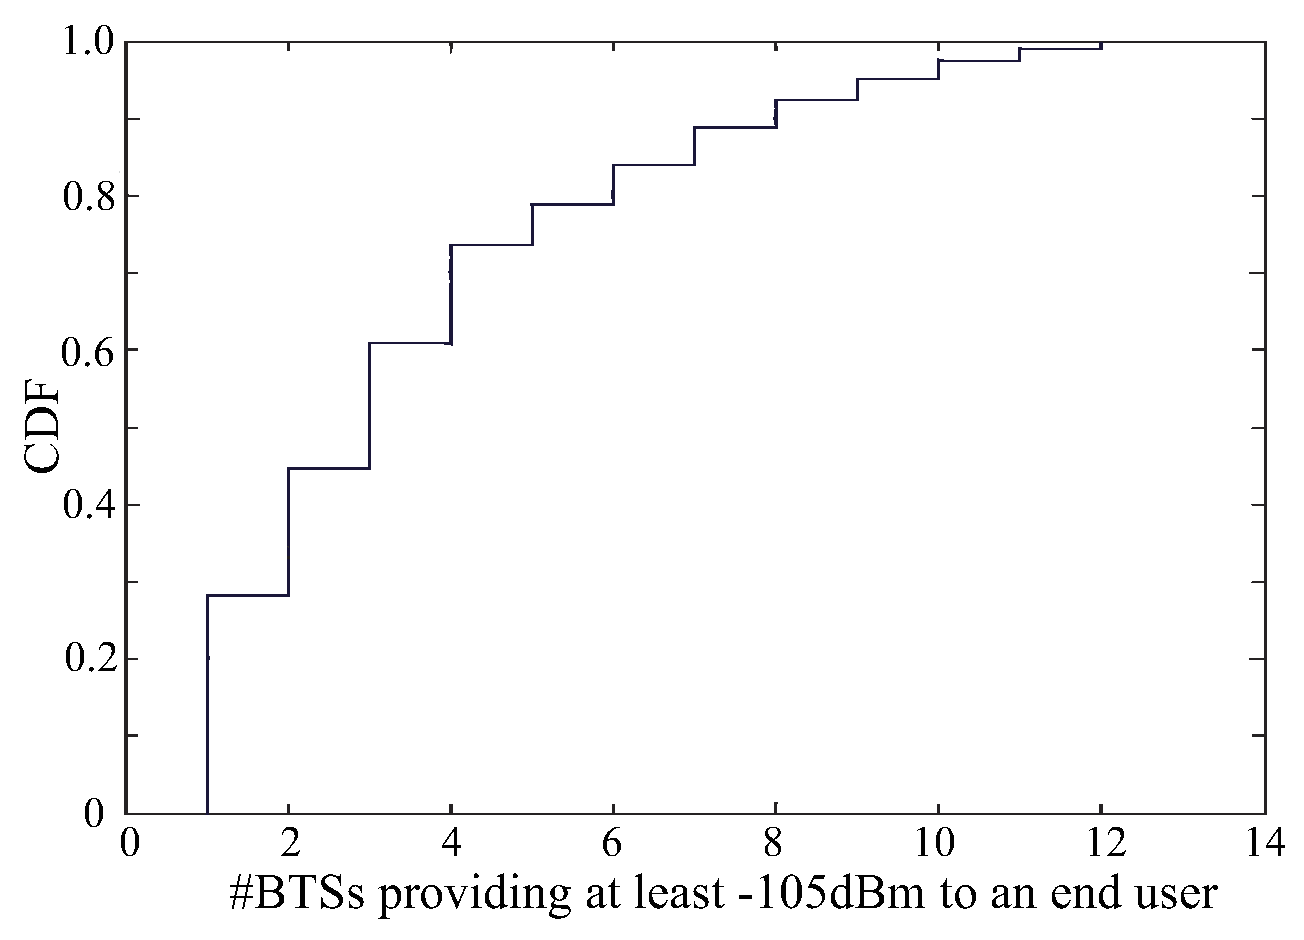
\includegraphics[width=0.8\textwidth]{pics/coveragecdf.eps}
\caption{Empirical CDF of the number of potential serving BTSs for a call in our dataset (large metropolitan area)}
\label{fig:btscdf}
}
\end{figure}

\begin{figure}
\centering
{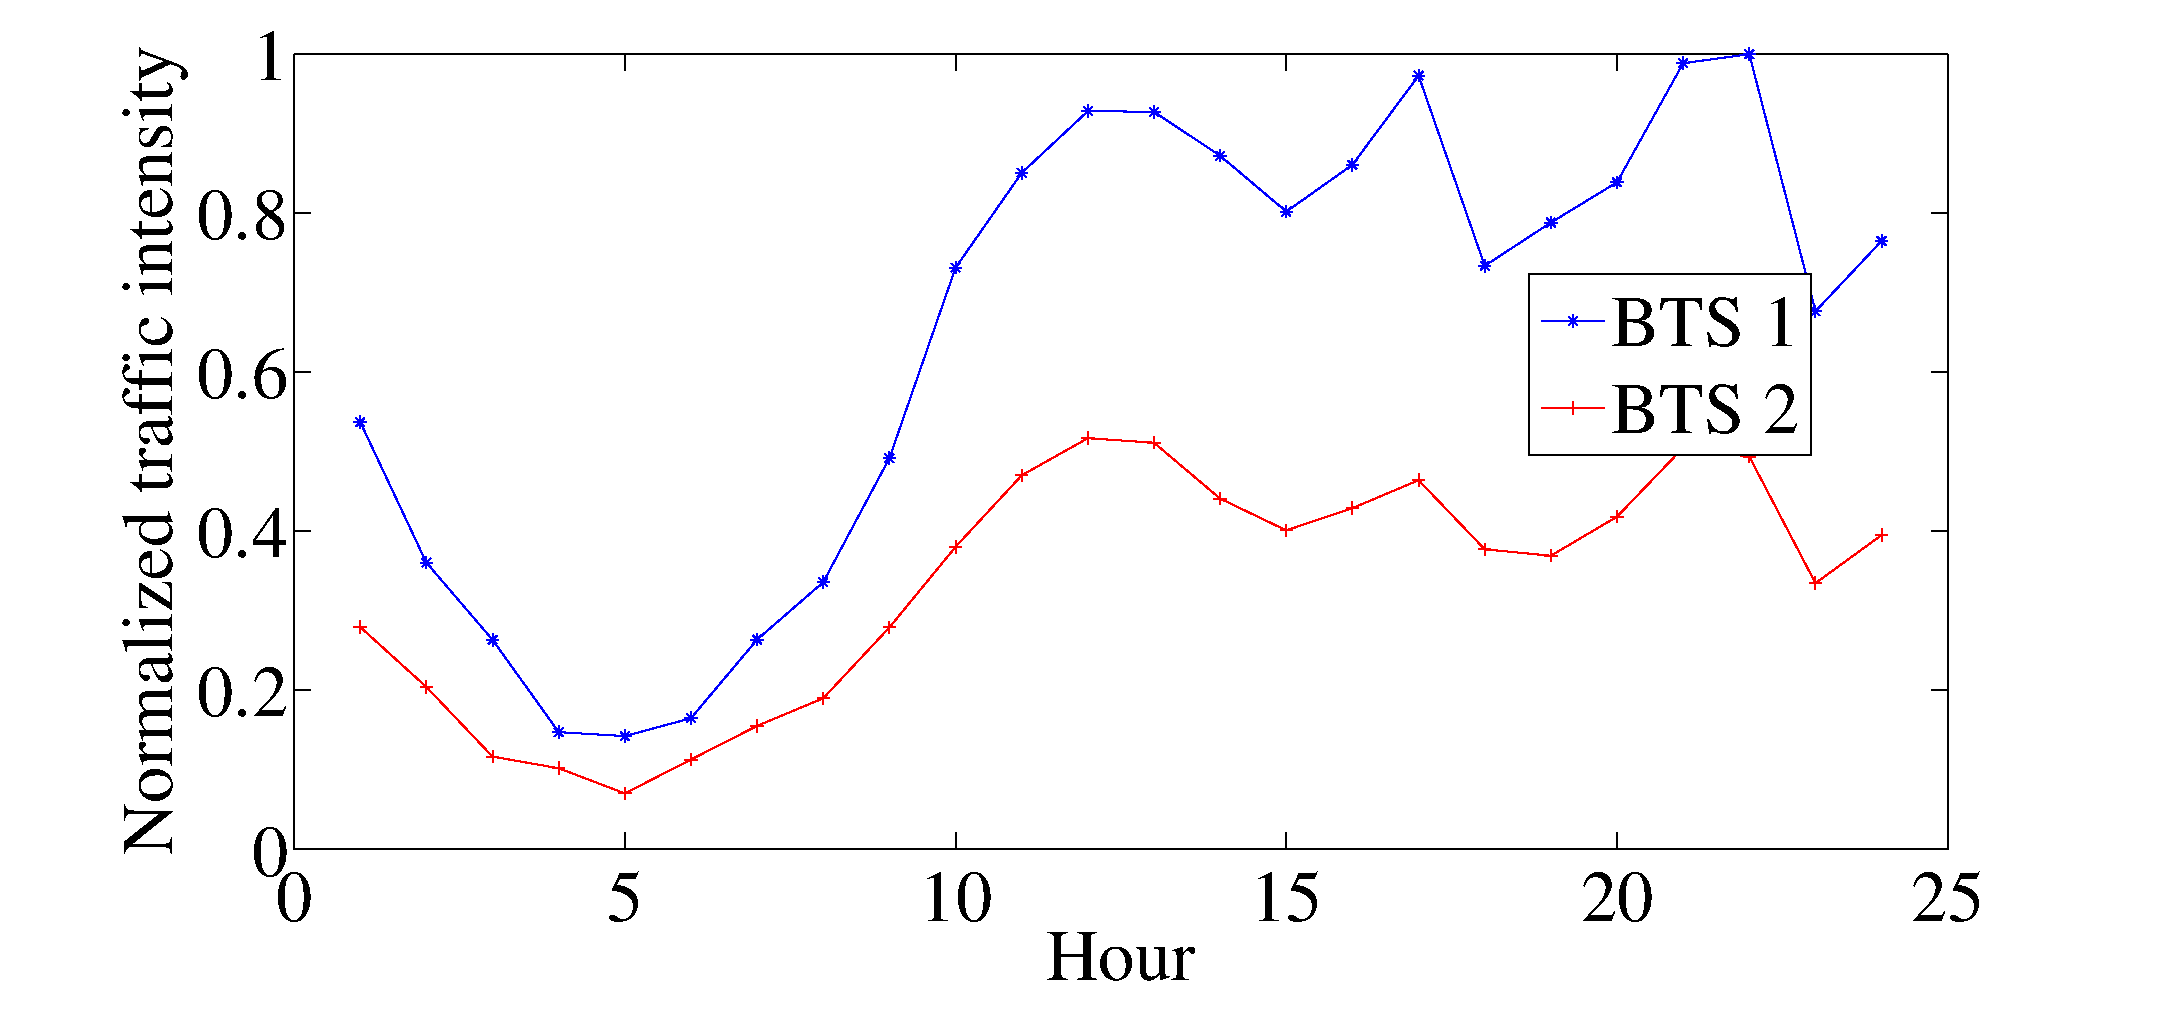
\includegraphics[width=0.8\textwidth]{pics/traffic.eps}
\caption{Normalized traffic for a 24-hour period at two neighboring sites in our dataset shows the geo-diversity in traffic}
\label{fig:traffic}
}
\end{figure}

\section{Related work}
\label{sec:case2:related}
One can improve the energy efficiency of a cellular network by
adapting its ``online'' capacity to changes in traffic load.
Recent work has proposed turning off base stations to reduce
energy consumption during times of low traffic
load~\cite{Louhi:2007:BTSPower:INTELEC,Oh:Comm:2011,Peng:2011:BTSSaving:Mobicom,He:CellularPower:JN:2012}.
In such solutions, to offer the same amount of coverage, the transmit range of some of the remaining BTSs has to be increased. Our conversations with multiple network operators
indicate that they are reluctant to employ such techniques
citing three reasons:
\begin{itemize}
\item Power cycling of entire base stations is expected to
    reduce equipment life time.
\item Turning off some BTSs may require an increased uplink
    power which may not be handled by many low-cost/power-limited mobile
    stations (MSs). This raises a risk of customer churn and is
    not acceptable to the operators in cut-throat
    competition prevalent in today's market.
\item These techniques of turning off BTSs may
    underestimate the increase in power needed for indoor
    MSs.
\end{itemize}

Our work is very similar in spirit to the concept of
\textit{frequency dimming}
in~\cite{Tipper:Dimming:Globecom:2010} albeit at a different
level of abstraction. A similar approach is also proposed
in~\cite{Blume:2010:BLTJ:CellularPower} with some rough
estimates of expected savings. We, on the other hand, use site
locations and traffic traces from a large cellular network with
more than 13 million subscribers to run a simulation study
assessing the benefits of dynamic equipment scaling coupled
with call hand-offs.
A key benefit of our approach is that it 
does not require any additional hardware
and works within the GSM specifications.

Much prior work focuses primarily on recent and future generation cellular networks such as WiMax and LTE. The operational nature of GSM, the focus of our thesis, is so different from these networks that the energy efficiency improvement techniques proposed for such networks do not apply to GSM. Nonetheless, in this section, we do touch upon some of the recent work on energy efficiency in non-GSM networks as well. In~\cite{Deruyck20112036}, Deruyck et. al. have proposed a useful metric, power consumption per covered area, to measure the energy efficiency of WiMax, fixed WiMax, UMTS, HSPA and LTE. The authors rank these networks in order of energy efficiency based on their proposed metric and also investigate the impact of MIMO on energy efficiency of these networks. Good surveys of BTS energy efficiency improvement techniques for 3G networks may be found in~\cite{6056687,5783984}.

Transmit power adjustment for BTSs is critical for the operation of networks such as CDMA and WiMax, as it determines the interference level in the cells. Several researchers have investigated optimal transmit power allocation techniques, for instance see~\cite{Kavitha20131373,Xu:powercontrol:2013}. Transmit power adjustment using cell-breathing was proposed in~\cite{Bhaumik:2010:BSC:1851290.1851300} with the objective of reducing energy consumption in 3G cellular networks. Han et. al. also proposed a cell-breathing based approach for cellular networks in the presence of green energy sources in~\cite{6189819}.

Small cells such as pico and femto cells are also gaining popularity due to better energy efficiency compared to large macro-cells. Such cells are generally deployed within large organization's premises to enhance indoor coverage without significant increase in transmit power. We have not considered this type of cells because our conversations with network operators revealed that they are not common in the developing world. The interested reader will find some investigation of energy efficiency improvement and power optimization in the presence of pico and femto cells can be found in~\cite{6576465,6491498} 

\section{Instantiating the generalized optimization formulation} %Derive the objective function and constraints. Clearly outline the assumptions that we've made about the geo-diverse data centers.
\label{sec:case2:instantiate}
The RED-BL optimization problem minimizes the sum of state and transition costs for a network over a sequence of consecutive intervals in a planning window. The state cost for a particular interval is the sum of electricity cost incurred at all BTSs in the network. In order to compute the state cost, we will first derive a mathematical model for electricity consumption at a single BTS. Then, we will generalize it to a multi-BTS cellular network setting to represent the state cost for a single interval. The transition cost would be the cost of electricity incurred in activating or deactivating TRXs. Our conversations with network operators reveal that transitions into and out of BTS Power Saving mode do not consume a noticeable amount of power. These state transitions are reasonably fast in contrast to the delayed convergence due to transitions in the geo-diverse data center scenario. The RED-BL transition costs in cellular networks may, therefore, be ignored.

\subsection{Single Base Transceiver Station (BTS)}
\label{sec:case2:instantiate:single-cell}
Power consumed by a BTS, as a function of traffic load, can be
well approximated as an affine function  of traffic volume~\cite{Peng:2011:BTSSaving:Mobicom} given as
$P_1+l(P_2-P_1)/t_{max}$. Here $P_1$ and $P_2$ are the power
consumption at no load and full load, respectively, $l$ is the
number of calls presently being handled, and $t_{max}$ is the
maximum number of simultaneous calls that can be handled.

Let $\delta$ be the traffic threshold below which the \textit{BTS power savings} may be applied (i.e., when BTS deactivates some TRXs moving into low-power mode). Since all TRXs are identical, the per call increase in power consumption, and hence the slope of the power consumption profile in Fig.~\ref{fig:powermodel}, remains the same in the default high-power mode, with all TRXs active, and the low-power mode, where some TRXs are deactivated. As also indicated in Fig.~\ref{fig:powermodel}, the no-load power consumption drops to $P_1-\gamma$ in the low-power mode, where $\gamma$ is a constant that depends on the equipment type and the number of TRXs deactivated. If $x$ is an indicator variable which is $0$ when \textit{BTS power savings} is applied, and $1$ otherwise, then the BTS power consumption may be given by $P_1+l(P_2-P_1)/t_{max} - (1-x)\gamma$ (indicated in Fig.~\ref{fig:powermodel} by the piecewise linear solid line).

\begin{figure}
\centering
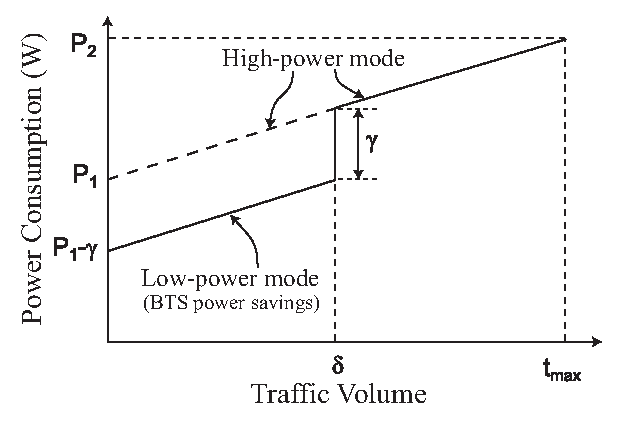
\includegraphics[width=0.8\textwidth]{pics/powermodel.eps}
\caption{BTS power consumption model. Low-power (BTS power savings) mode is optional and kicks in at low loads.}
\label{fig:powermodel}
\end{figure}

\begin{figure}
\centering
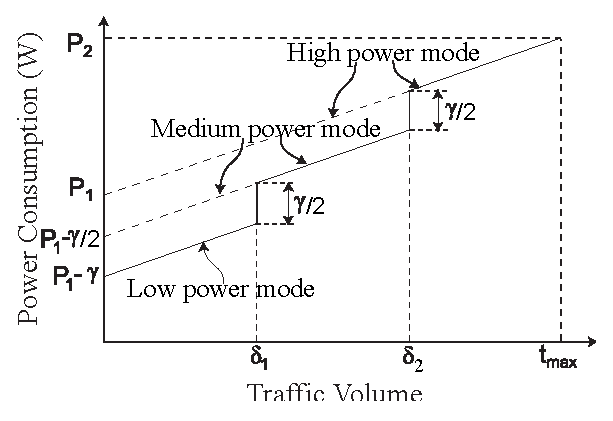
\includegraphics[width=0.8\textwidth]{pics/powermodel2-1.eps}
\caption{BTS power consumption model with finer granularity of BTS power saving.}
\label{fig:powermodel2}
\end{figure}

The BTS equipment may be configurable in more than two-states, depending on the available granularity of TRX deactivation. for instance, a three-state BTS power consumption model is shown in Figure~\ref{fig:powermodel2}. If the traffic is above threshold $\delta_2$, the BTS operates in the default high-power mode. When the traffic drops below threshold $\delta_2$, two TRXs per sector are deactivated, and the BTS enter the medium-power mode (4+4+4 configuration). When the traffic falls below threshold $\delta_1$, two more TRXs are deactivated and the BTS enters the low-power mode. The drop in power consumption for each of the deactivation steps is $\gamma/2$, because compared to Figure~\ref{fig:powermodel1}, half as many TRXs are deactivated in each step.

If traffic load is $\delta + \epsilon$ then the less granular model of Figure~\ref{fig:powermodel1} does not offer any energy savings but the more granular model ofFigure~\ref{fig:powermodel2} offers an energy saving of $\gamma/2$. The more granular model of Figure~\ref{fig:powermodel2} should, therefore, offer greater energy savings overall. We will show later that this greater energy saving is at the cost of increased complexity of the optimization problem.  

\subsection{Multi-BTS Cellular Setting}
\label{subsec:case2:instantiate:multi-cell}
Consider an area with $n$ active callers being served by $m$ BTSs. We introduce indicator variable $w_{i,j}$, which is $1$ if call $i$ \textit{is being} handled at BTS $j$ and $0$ otherwise. We assume availability of an $n\times m$ matrix whose entry $c_{i,j}$ is $1$ if caller $i$ \textit{can be} served through
BTS $j$ without exceeding the uplink or downlink budgets. This information can be extracted by the data periodically transmitted by each MS comprising the received signal strength from nearby BTSs during a call. We also introduce indicator variable $x_j$, which is $1$ if BTS $j$ is operating in high-power mode and $0$ otherwise. The total power consumption may, therefore, be given as $\sum_{j=1}^{m} \left[P_1+\sum_{i=1}^{n}\frac{w_{i,j}(P_2-P_1)}{t_{max}}-(1-x_j)\gamma\right]$. Using this as the objective function, we can formulate the Low-Carb optimization problem as:
\begin{align}
\textit{minimize} \quad \sum_{j=1}^{m} \left[
P_1+\sum_{i=1}^{n}\frac{w_{i,j}(P_2-P_1)}{t_{max}}-(1-x_j)\gamma
\right]
\end{align}

subject to the following constraints:
\begin{align}
& \sum_{j=1}^m w_{i,j} = 1 \qquad \forall i \\
& w_{i,j} \leq c_{i,j} \qquad \forall i, j \\
& \sum_{i=1}^nw_{i,j}-\delta + \epsilon \leq Mx_j \qquad \forall j \\
& \sum_{i=1}^n w_{i,j} \le t_{max} \qquad \forall i \\
& w_{i,j}, x_j \in \{0,1\} \qquad \forall i, j%\\
\end{align}

The first constraint ensures that no active call is
dropped just to save on power. The second constraint secures
the uplink budget by ensuring that no call is routed to a BTS
that is too far away. The third constraint picks the correct
value for the decision variable $x_j$ ($M$ is a very large integer constant). The fourth constraint is the BTS capacity constraint, while the last
constraint is the binary value constraint on the decision
variables.

Constant additive terms play no role in an optimization objective function and may be omitted. The first term ($P_1$) can, therefore, be be dropped from the objective function. Furthermore, in order to not affect the grade of service, we will not drop any active calls. Hence, the summation over $w_{i,j}$ is also constant and can also be excluded from the objective function. After removing the constant multiplier from the last remaining term in the objective function, it reduces to:
\begin{align}
\textit{minimize} \quad \sum_{j=1}^{m} x_j
\end{align}

\subsubsection{Problem complexity}
\label{subsubsec:lowcarb:complexity}
We will now show that the above optimization problem, which we call Low-Carb (short for Lower Carbon footprint), is NP-Hard. Suppose that there exists and algorithm that gives a polynomial running time optimal solution to Low-Carb. We will prove that this assumption is wrong by mapping an NP-Hard problem to Low-Carb. 

The Low-Carb problem itself can be shown as NP-Hard by mapping the multiple knapsacks problem~\cite{kellerer:knapsackproblems:2005} to it. Our formulation itself is an NP-Hard Binary Integer Program
(BIP), making it intractable to solve for an
operator's entire network. It could, however, be applied separately to small disjoint network segments. Alternatively, a heuristic solution, such as the one we present in Algorithm~\ref{algo:heur2}, could be deployed over the entire network.

Our heuristic first partitions the set of BTSs $B$ into disjoint sets $B_1$ and $B_2$ where the latter includes all the BTSs in low-power mode and the former consists of all other BTSs. The heuristic iterates over a random permutation of the BTSs in $B_1$. Once a BTS $b_j$ from $B_1$ is selected (line 3), we determines the minimum number of calls that must be handed off from $b_j$ before it can be moved to $B_2$. We iterate over the calls being handled by $b_j$ and for each such call we try to find a candidate serving BTS in $B_2$ that may handle another call without leaving $B_2$. If such a BTS is found, the call is handed off to it. Calls are handed off from $b_j$ in this manner, until it moves into $B_2$, or we exhaust the set of active calls with other candidate BTSs ($b_j$ remains in $B_1$). 

\begin{algorithm}
\caption{Heuristic for the Low-Carb problem}
\label{algo:heur2}
\begin{algorithmic}[1]
\REQUIRE $\delta$: the power-saving traffic threshold,\\B (the set of BTSs) =\{$b_1, b_2, ..., b_m$\},\\A (the set of active calls) =\{$a_1, a_2, ..., a_n$\},\\W (current call association) =\{$w_{i,j}$ = 1 if $a_i$ is being served through $b_j$, 0 otherwise\},\\C (Possible call association matrix) = \{$c_{i,j}$ = 1 if $a_i$ \\can be served through $b_j$, 0 otherwise\}
\ENSURE A new and potentially more energy efficient mapping of calls to BTSs
\STATE $B_1$ = random\_shuffle($\{b_j | \sum\limits_{i=1}^{n}w_{i,j}>\delta\}$); 
\STATE $B_2=B - B_1$
\FORALL{$b_j \in B_1$}
	\STATE $\gamma$ = $\sum\limits_{i=1}^{n}w_{i,j} - \delta$; \quad shuffled = 0;
	\STATE $A^j$ = $\{a_i | w_{i,j}=1\}$; \quad shuffled = 0;
	\FORALL{$a_k \in A^j$}
		\IF{shuffled $< \gamma$}
			\STATE $B_2^k = \{b_p | c_{k,p}=1, b_p \in B_2\}$;
			\FORALL{$b_p \in B_2^k$}
				\IF{$\sum_{q=1}^n w_{q,p} < \delta$}
					\STATE $w_{k,q} = 1$; \quad shuffled++;
					\STATE $w_{k,j} = 0$; \quad break;
				\ENDIF
			\ENDFOR
		\ENDIF
	\ENDFOR
	\IF{$\sum\limits_{i=1}^n w_{i,j} \le \delta$}
\STATE $B_1 = B_1 - \{b_j\}$; \quad $B_2 = B_2 + \{b_j\}$
\ENDIF
\ENDFOR
\end{algorithmic}
\end{algorithm}

\subsection{Multi-level BTS scaling}
\label{subsec:case2:multilevel}
For the three-step BTS power-saving model of Figure~\ref{fig:powermodel2}, the optimization problem can be stated as:
\begin{align}
\textit{maximize} \quad \sum_{j=1}^{m} \left[
x_j+y_j
\right]
\end{align}
subject to the following constraints:
\begin{align}
& \sum_{j=1}^m w_{i,j} = 1 \qquad \forall i \\
& w_{i,j} \leq c_{i,j} \qquad \forall i, j \\
& \sum_{i=1}^nw_{i,j}-\delta_1 \leq Mx_j \qquad \forall j\\
& \sum_{i=1}^nw_{i,j}-\delta_2 \leq My_j \qquad \forall j\\
%\end{align}
%\begin{align}
& \sum_{i=1}^n w_{i,j} \le t_{max} \qquad \forall i \\
%\end{align}
%\begin{align}
& w_{i,j}, x_j, y_j\in {0,1} \qquad \forall i, j%\\
%x_j \in {0,1}
\end{align}

In the above formulation, we've added an indicator variable $y_j$, which is $1$ if BTS $j$ is in medium-power mode, $0$ otherwise. The fourth constraints ensures that $y_j$ takes on the proper value depending on the current traffic volume at BTS $j$. We call this optimization problem the three-step Low-Carb problem.

Adding a granularity level introduces $m$ additional binary variables causing the solution space to grow by a factor of $2^m$. At the same time, $O(m)$ constraints are also added to the problem. Binary Integer Programming problems such as ours are NP-Hard. While solutions to small-sized problems may be obtained in a reasonable period of time, but it lacks scalability. Therefore, increasing the number of BTS operating modes causes an exponential increase in the execution time to obtain an optimal solution. 

For ease of modeling and implementation, we assume that all sectors will be configured to have the same number of TRXs active at any given time. Thus a 6+6+6 site may have six possible states, 1+1+1, 2+2+2, ..., and 6+6+6. To develop the optimization model for a six-state BTS, consider an integer variable $z_j$ which represents the number of TRXs active in each sector of BTS $j$. The power consumption at BTS $j$ may be given by $P_1 + p \sum_{i=1}^{n} w_{i,j} + \gamma z_j$, where p is the slope of the power consumption vs traffic volume curve. The Low-Carb optimization problem for the multi-BTS setting in this case is:

\begin{align}
\textit{minimize} \quad \sum_{j=1}^{m} z_j
\end{align}
subject to the following constraints:
\begin{align}
& \sum_{j=1}^m w_{i,j} = 1 \qquad \forall i \\
& w_{i,j} \leq c_{i,j} \qquad \forall i, j \\
& \sum_{i=1}^nw_{i,j}-\delta_1 +\epsilon \leq Mz_j \qquad \forall j \\
& \sum_{i=1}^n w_{i,j} \le t_{max} \qquad \forall i \\
& w_{i,j} \in \{0,1\}; \quad z_j \in \{1,2,3,4,5,6\}\qquad \forall i, j%\\
\end{align}

The first constraint ensures that each call is handled at exactly one BTS. The second one ensures that a call is mapped to a BTS that may handle it. The third constraint ensures that $z_j$ picks a value at least equal to the minimum number of TRXs required at BTS $j$. Since the optimization is a minimization problem, the solver will pick $z_j$ to be exactly equal to the minimum number of TRXs required for the current traffic load. The fourth constraint is the capacity constraint on the BTS. The last set of constraints specify the domains of the decision variables.

\section{Experimental setup} 
\label{sec:case2:experiments} Our dataset is obtained from a cluster of 26 BTSs operated by a large network operator with more than 7000 sites. These sites are spread over a $31.25$ $km^2$ urban terrain (see Fig.~\ref{fig:sites}). We obtained each site's coverage prediction using a tool popular amongst the operators called Forsk Atoll. With this information, alongwith a caller's location, we can determine the candidate set of BTSs for the corresponding call (the $c_{i,j}$ parameters). Note that in this thesis, we do not incorporate user mobility into our model, since we are only interested in instantaneous optimization at small time scales and in determining bounds on the energy savings that Low-Carb can offer.

Also available to us are the hourly cumulative traffic, in Erlang, for each of the sites, spanning two consecutive weekdays. The traffic remained remarkably similar across both days for each site. We have, therefore, only used one day's traffic data in our experiments.

Using the above datasets, we conducted a set of experiments mimicking a 24-hour operation of a subset of a cellular network. Each experiment is a discrete event simulation of the arrival and placement of calls. Since our dataset does not include the arrival times and duration of calls, we synthetically generated this information using the assumption of Poisson call arrivals and exponentially distributed call duration with a mean of $180$ seconds~\cite{Gerla:1995:MMM:276418.276421}.

For every hour, the simulator determines the Poisson call arrival rate for each BTS, using Little's Law and the BTSs traffic intensity for that hour. Using the resulting Poisson process, calls are generated such that it is equally likely for a call to be anywhere in the serving BTSs coverage area.

Our simulator tracks the call volume at every BTS on a minute's granularity, thereby computing a time series of the power consumption (in Watts) for each BTS. This enables it to calculate three values. First, it accumulates the power consumption for each BTS over the 24 hour period, thereby computing the daily amount of energy consumed (in kWh) if no optimization is used in the network. Second, by identifying low-traffic episodes for each BTS the simulator selectively places some BTSs in power-saving mode, thereby computing the possible energy savings using BTS power-saving feature. Third, our simulator also periodically determines the instantaneous optimal call placement configuration using call hand-off, such that a maximal number of BTSs are placed in power-saving mode, thereby determining the optimal energy savings by coordinated call hand-offs and BTS power-saving.

The call placement re-optimization may be done at various frequencies. A very aggressive re-optimization regime would keep the network in an optimal state more often than a conservative one, thereby enabling greater energy savings. In order to study the scaling of energy saving with re-optimization frequency, we experimented with a range of intervals between successive optimizations, ranging from a minute to an hour. For a deployment, the re-optimization frequency that can be used would depend on the costs associated with each re-optimization. Let us now consider such costs.

First and foremost, a computational cost is incurred with each optimization. For our dataset, an optimization run to determine the optimal state over $26$ BTSs required an average running time of about $50$ seconds on a Core i3 laptop with 4 GB of RAM. An optimization requiring $50$ seconds would not be practical to use every minute but may be fine if used less often. For a practical deployment the computational time can be reduced by using a combination of a more powerful machine, distributed optimization and approximation algorithms. 

In addition to the computational overhead, for every unit of energy saved some extra energy may be consumed in the network to perform call hand-offs or transitions into and out of BTS power-saving mode. Call hand-offs and TRX (de)activation involve signaling between a Base Station Controller (BSC), BTSs and MSs. The additional energy incurred thus, should be small, because it has been observed that variation in power consumption of network equipment with changes in traffic volume (data or control) is quite small~\cite{Chabarek08powerawareness}. As far as increased power consumption on MSs due to a greater number of call hand-offs is concerned, we opine that it may be negligible because the MSs energy consumption is far outweighed by that of BTSs.

\subsection{Site Characteristics}
\label{subsec:case2:experiments:sitetypes} All sites in our dataset had three sectors, each equipped with 6 TRXs, for a maximum of 132 simultaneous voice calls\footnote[1]{Each TRX's frequency is shared in time-domain  by 8 calls for  a total of $3\times6\times8=144$ channels. Four channels in each sector were reserved for control and broadcast purposes.}. The GSM standard includes a provision for half-rate calls, which enables handling greater traffic at the expense of reduced voice quality by allowing a single voice channel to be shared amongst two calls, each using a half-rate codec. In this thesis, we only shuffle full-rate calls around, which may be, in reality, two half-rate calls. We do not foresee any significant error arising from using this convention.

We consider a scaling down from a $``6+6+6"$ site to a $``2+2+2"$ site, which means that $\delta$ should be strictly less than $t_{max}/3$ to avoid quick oscillations into and out of BTS power-saving mode due to short-term traffic variations. We have arbitrarily set $\delta$ equal to $\lceil t_{max}/3\rceil -5$, because $5$ seemed to be a good enough number compared to a sector's overall capacity and the typical utilization of a site in our datasets.

The BTS power consumption model parameters may vary from one BTS model to another. In this thesis, we use three different sets of model parameters as listed in table~\ref{tab:models}. We now describe the sources and methods from which we obtained these models.
\subsubsection{Model 1}
\label{subsubsec:case2:experiments:sitetypes:model1}For the first model, we have used $1.5kW$ as the maximum power consumption~\cite{mbakwe:btshybribpower:2011:necec}, a $20W$ per TRX saving when scaling the BTS down~\cite{flexibsc} and a $5\%$ swing in power consumption between no-load and full-load~\cite{Peng:2011:BTSSaving:Mobicom}.

\subsubsection{Model 2}
\label{subsubsec:case2:experiments:sitetypes:model2} Lorincz et. al reported the single sector DC power consumption for a GSM 900 BTS with 7 TRXs~\cite{Lorincz:BTS-Measure:Sensors:2012}. We extrapolate the power consumption for a 6+6+6 site by multiplication of the DC power consumption reported in ~\cite{Lorincz:BTS-Measure:Sensors:2012} by $3\times6/7$. The DC power consumption does not include the AC power consumed in the power supply units and in air-conditioning. We must, therefore, also compensate for those to obtain the overall site power consumption. Power supply unit load is negligible compared to air-conditioning, which has a typical power consumption of 1 kW~\cite{mbakwe:btshybribpower:2011:necec}. We used this scaling and AC load correction to obtain the values for $P_1$ and $P_2$ using the minimum and maximum reported power consumption in ~\cite{Lorincz:BTS-Measure:Sensors:2012}. Furthermore, the authors in~\cite{Lorincz:BTS-Measure:Sensors:2012} measured a drop of $50W$ in power consumption when a TRX is disable, which gives us the value of $\gamma$ as listed in table~\ref{tab:models}.

\subsubsection{Model 3}
\label{subsubsec:case2:experiments:sitetypes:model3}Using the same method as for model 2 in~\ref{subsubsec:case2:experiments:sitetypes:model2}, we derived the values for $P_1$ and $P_2$ based on the measurements for a GSM 1800 BTS reported in~\cite{Lorincz:BTS-Measure:Sensors:2012}. As for the value of $\gamma$, the paper reported a $100W$ cut in power consumption when deactivating a single TRX. The parameter values for this model are given in Table~\ref{tab:models}

\begin{table}
\centering
\begin{tabular}{|c|c|c|c|}
\hline
Parameter & \multicolumn{3}{|c|} {Value} \\
\cline{2-4} \ & Model 1 & Model 2 & Model 3 \\
\hline $P_1$ & 1425 & 2401.8 & 2341.5 \\
\hline $P_2$ & 1500 & 3887.5 & 2973.9 \\
\hline $\gamma$ & 240 & 600 & 1200 \\
\hline
\end{tabular}
\caption{BTS model parameter values}
\label{tab:models}
\end{table}

\section{Results}
First, we consider the benefit of BTS power-saving alone, resulting from traffic diversity at each BTS compared to running the network in the default configuration. The percentage reduction in energy consumption is listed in TABLE~\ref{tab:psonly}. The results indicate that a saving of between 4\% and 12\% can be achieved in a network just by enabling BTS power savings. We note here that these results are in agreement with Ericsson's claim of saving 10-20\% energy by using BTS power-saving on Germany's Vodafone network~\cite{ericssonclaim}. 

In absolute terms, this represents a cumulative saving of between 43 kWh and 217 kWh per day over a set of 26 BTSs. Now, consider that there are five cellular operators in Pakistan: Mobilink with more than 8500 sites~\cite{mobilinksitecount}, Ufone with more than 8000 sites~\cite{ptaannreport}, Zong with more than 5500 sites~\cite{ptaannreport}, Telenor with more than 7000 sites~\cite{telenorsitecount} and Warid with more than 4500 sites~\cite{ptaannreport}. Overall, there were more than 31000 sites in Pakistan at the end of 2011. Extrapolating our experimental results suggests that a significant reduction in energy consumption is possible country-wide in Pakistan (and any other country with similar deployment and traffic characteristics) by just deploying BTS power-saving. This is especially significant for an energy-starved developing country. As we shall see next, greater energy savings are possible if we couple periodical call shuffling with BTS power savings in the network. 

\begin{table}
\centering
\begin{tabular}{|c|c|c|c|}
\hline Energy saving & Model 1 & Model 2 & Model 3 \\
\hline Percentage & 4.73\% & 5.43\% & 12.89\% \\
\hline Daily absolute saving & 43.28 & 109.68 & 217.12 \\
over 26 BTSs (in kWh) & \ & \ & \ \\
\hline Country-wide daily saving & 51.6 & 130.77 & 258.87\\
over 31000 sites (in MWh) & \ & \ & \ \\
\hline
\end{tabular}
\caption{Energy savings by using BTS power savings only}
\label{tab:psonly}
\end{table}

\subsection{Sensitivity of electricity cost savings to the duration of an optimization interval} Fig.~\ref{fig:case2:results2} shows the percentage energy savings achievable by coordinated call handoff and BTS power saving. Notice that if the interval between consecutive optimizations is greater than the mean call duration of 6 minutes, the percentage savings don't change significantly, whereas for shorter inter-optimization intervals, the percentage savings rise sharply. This is due to the fact that if re-optimization is performed at a rate faster than the mean call duration, a greater number of calls is routed optimally at least once during their lifetime. 

Since the three BTS models have quite different power consumption characteristics, percentage energy savings do not provide a useful metric for comparison of the relative utility of Low-Carb for these BTS models. We, therefore, also plot the absolute energy savings (in kWh) for each of the BTS models in Figure~\ref{fig:case2:results3}. For all three BTS models, we see the same trend in absolute energy savings as that in case of percentage energy savings. 

\begin{figure}
\centering
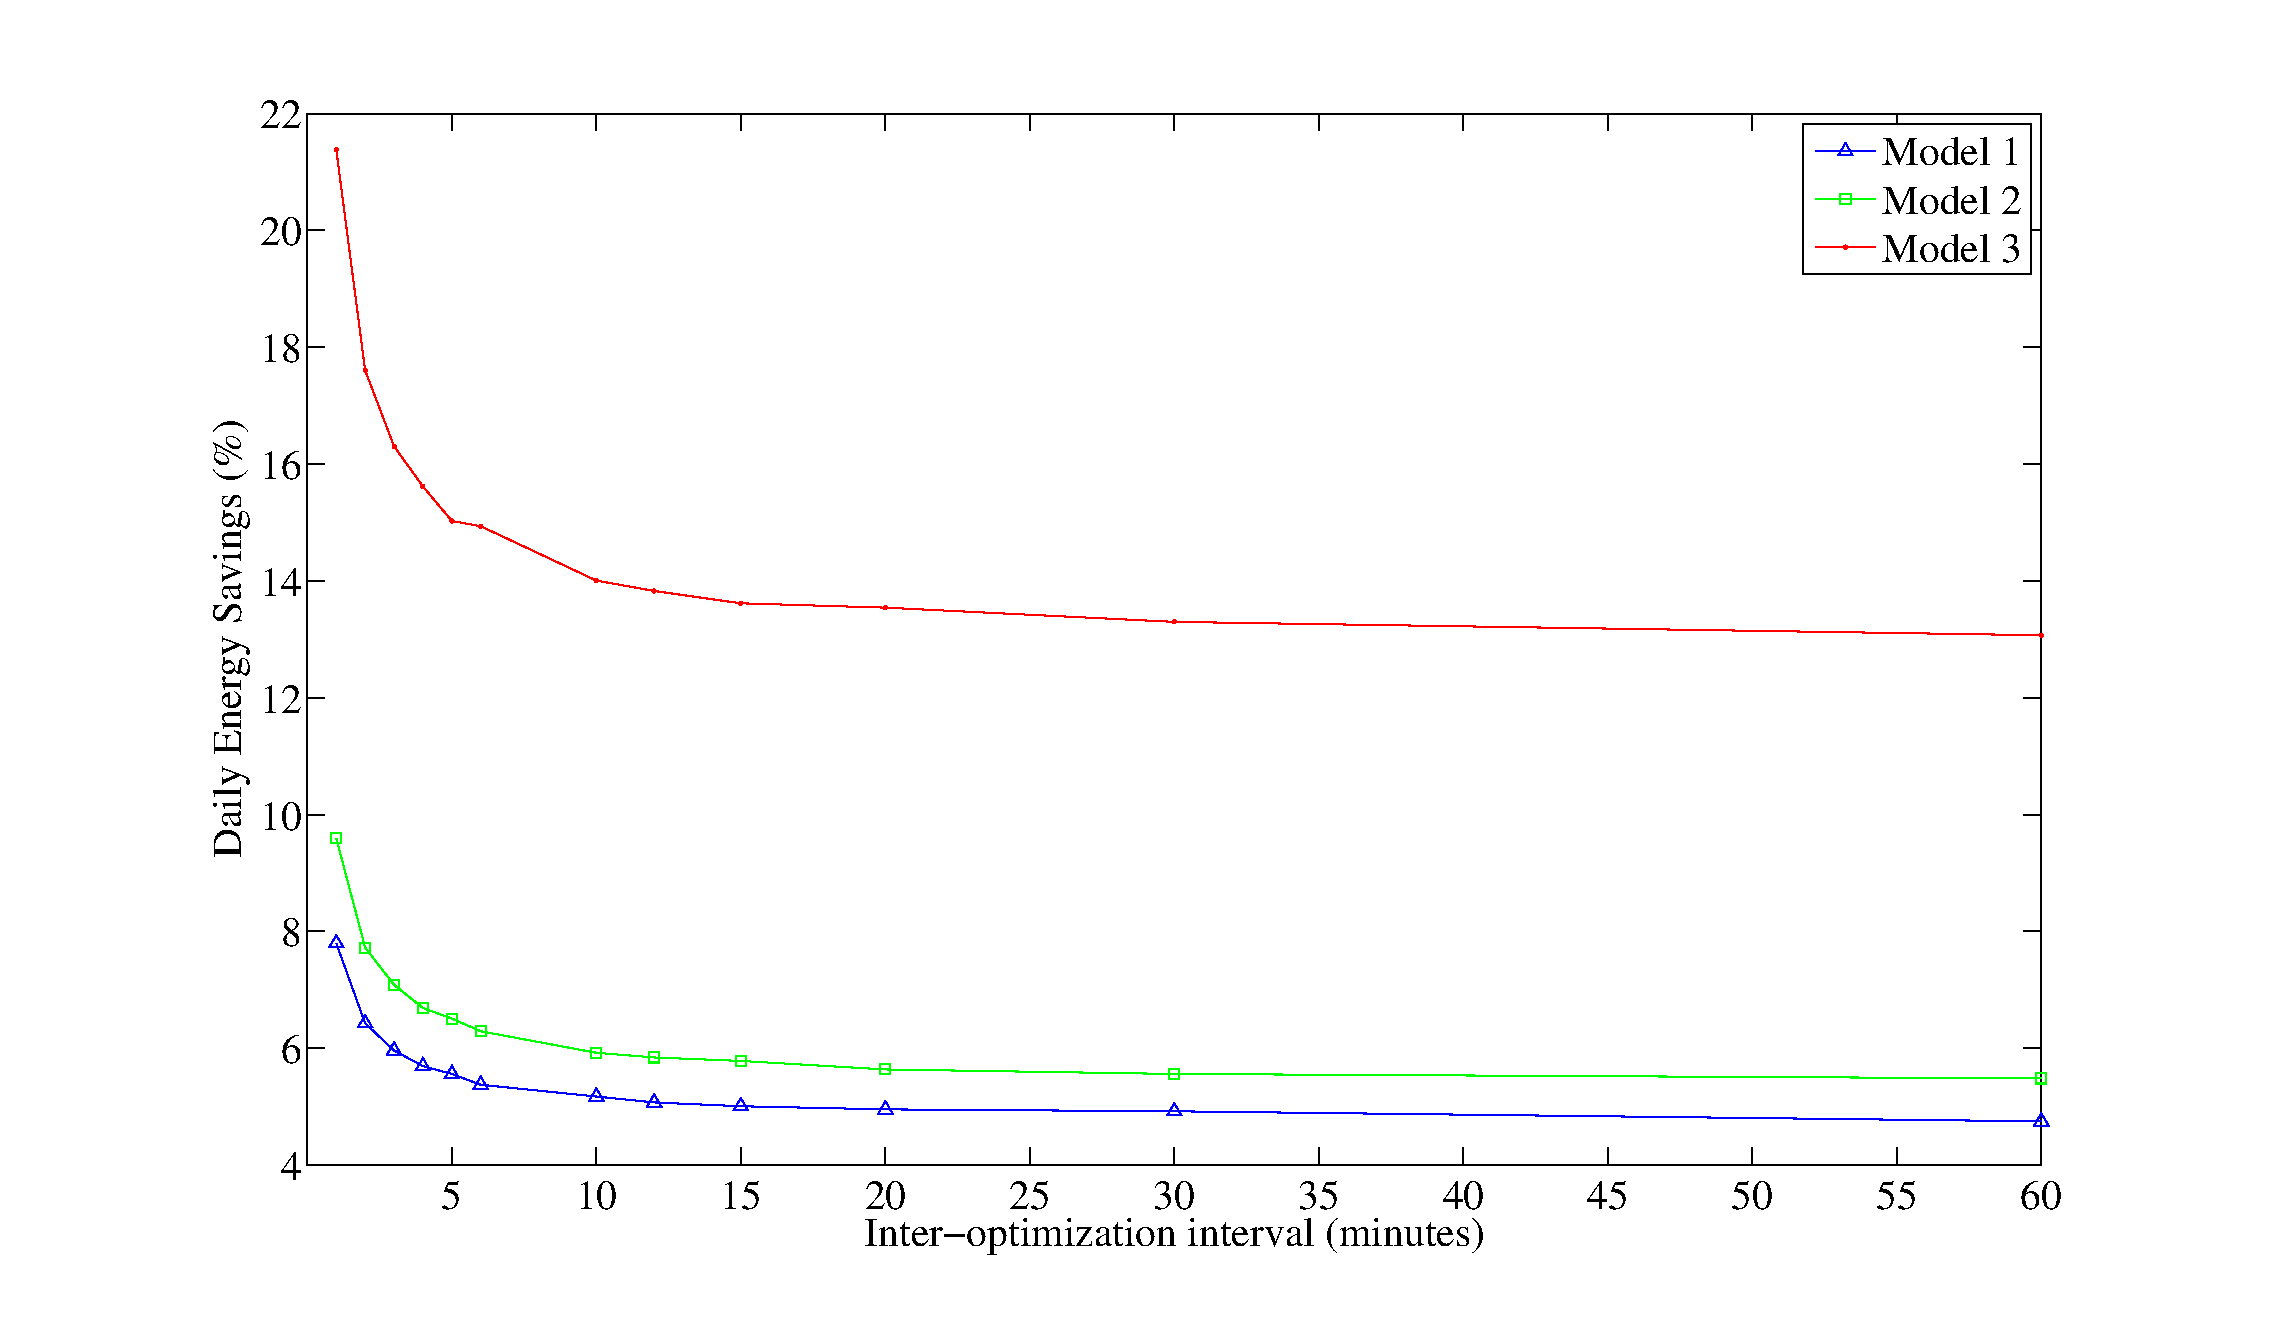
\includegraphics[width=0.8\textwidth]{pics/perc.savings.red-bl.eps}
\caption{Percentage reduction in energy consumption vs inter-optimization interval}
\label{fig:case2:results2}
\end{figure}

\begin{figure}
\centering
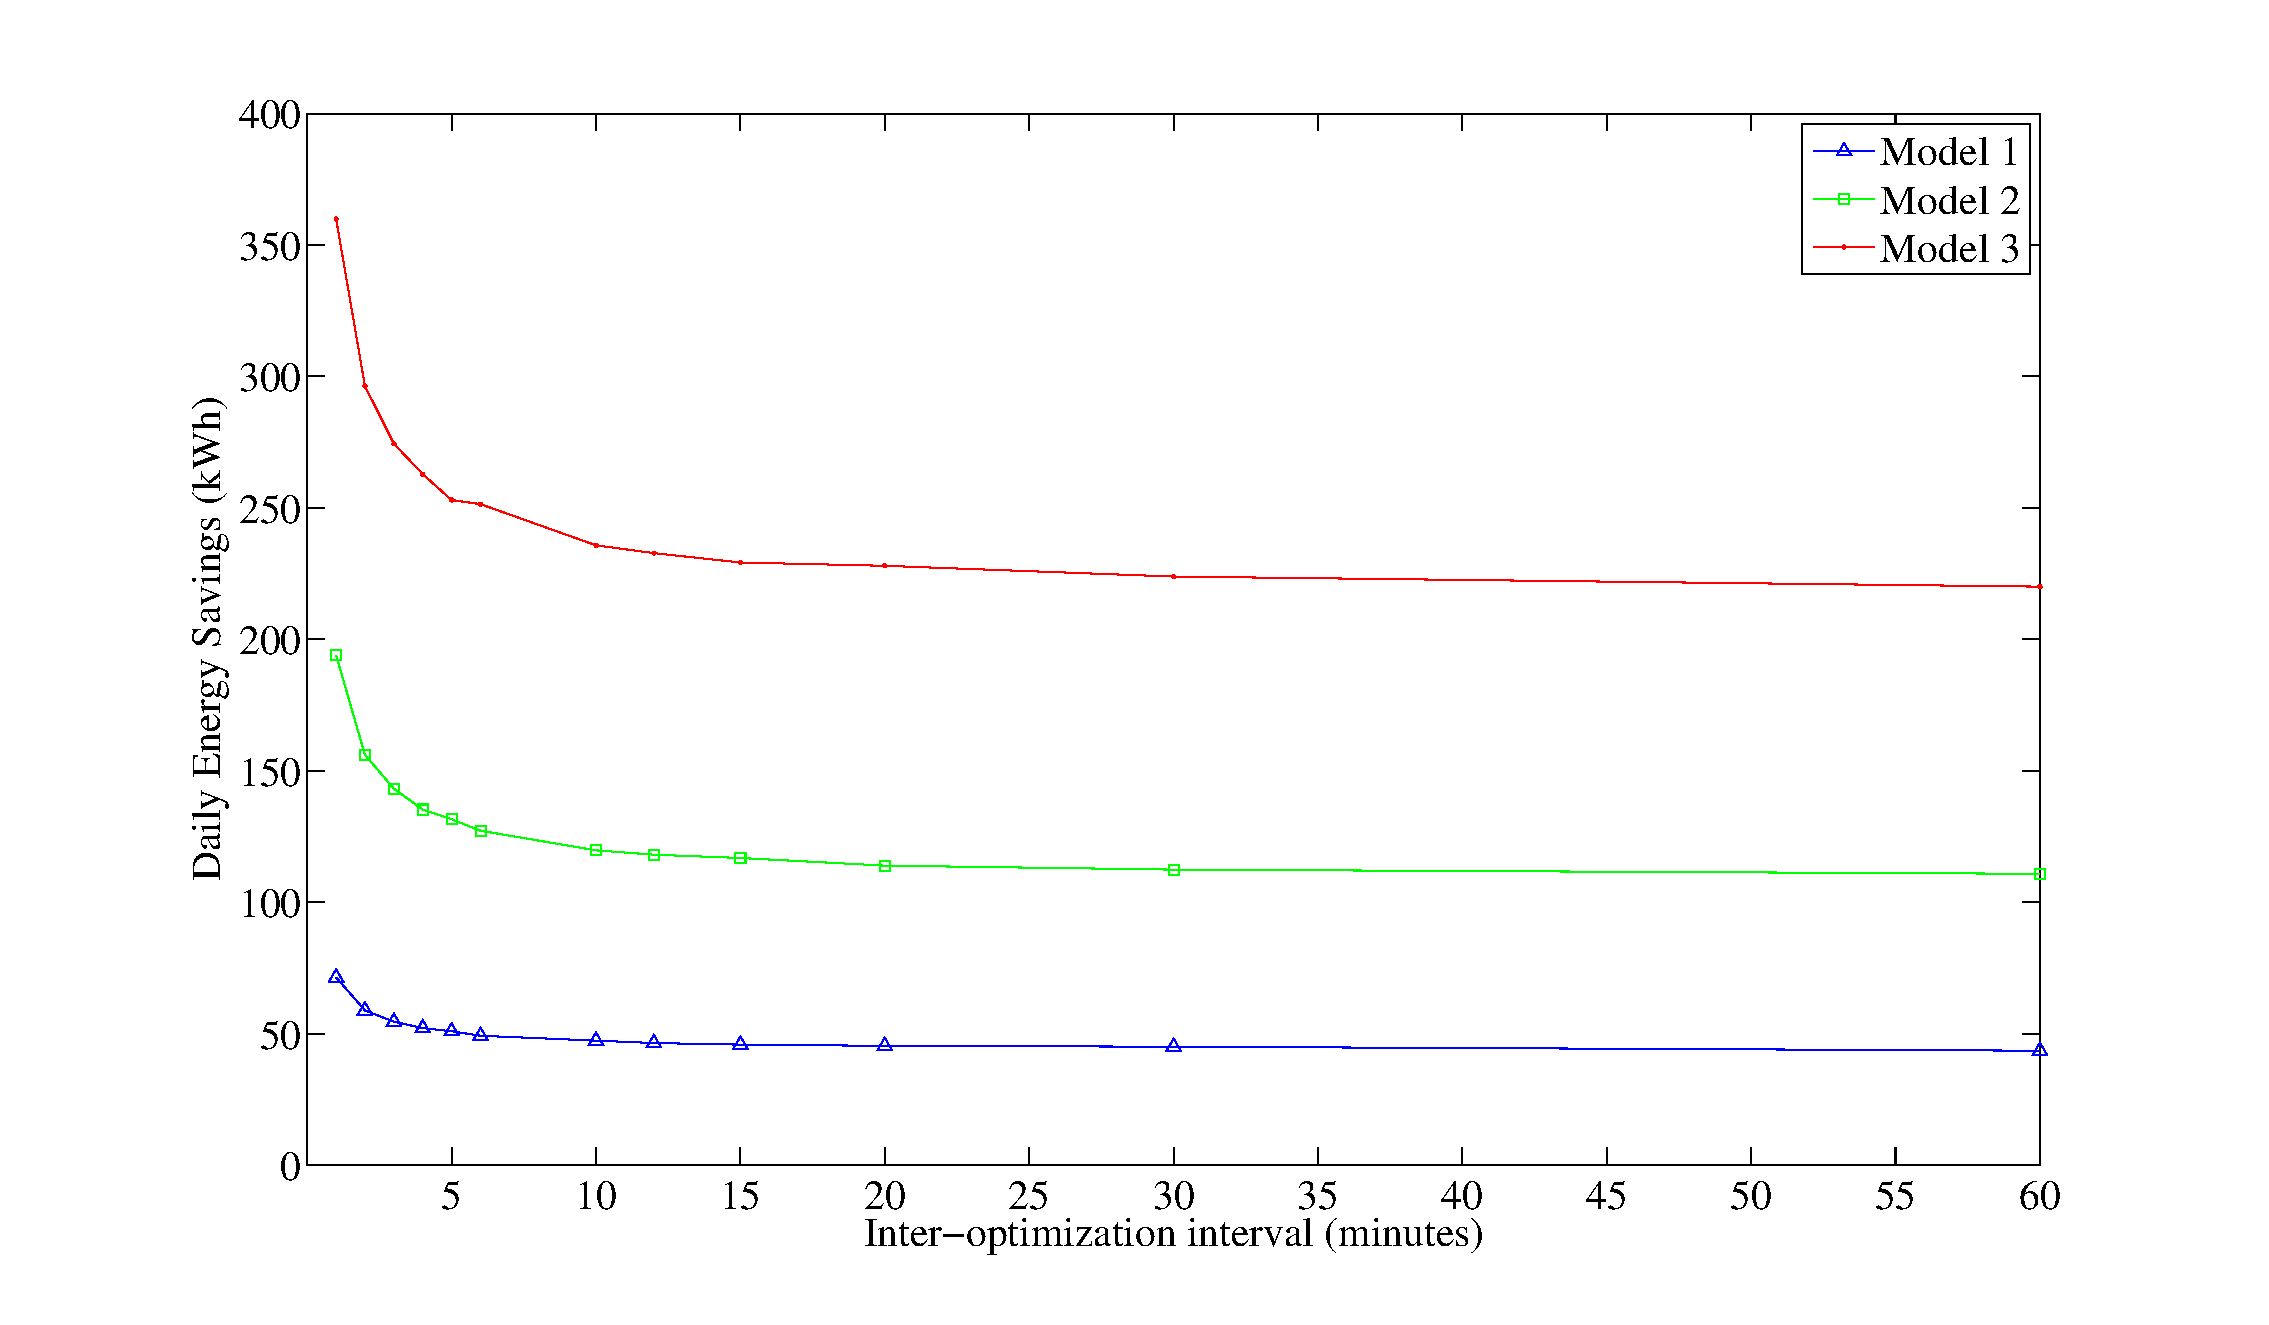
\includegraphics[width=0.8\textwidth]{pics/e.savings.red-bl.eps}
\caption{Percentage reduction in energy consumption vs inter-optimization interval}
\label{fig:case2:results3}
\end{figure}

%Re-optimizing at an interval less than the mean call duration should offer greater savings than a less frequent re-optimization. This is because the former regime has the ability to optimally hand off most of the calls at least once. Our results confirm this intuition. For model 1 BTS, for instance, the gain in energy savings while going from a 60 minutes re-optimization interval to 30 minutes is merely 0.0506 kWh per minute, whereas it is 15.5421kWh when decreasing the re-optimization interval from 2 minutes to 1 minute.

Let us now interpret what these results mean physically in terms of ecological impact. An extrapolation of our results indicates that for Pakistan, Low-Carb offers a total energy saving of $60.72$ MWh, $156.84$ MWh or $301.61$ MWh daily, respectively for each of the BTS models. For a small and energy-starved developing country, these energy savings are significant. Since network deployments and traffic patterns are similar in different countries, the same extrapolation can be applied to other countries as well.

In the above extrapolation, we have assumed that the same amount of energy saving would be applicable in rural as well as urban settings. One may argue that in rural settings, due to sparse deployments the energy savings potential would be lower because few calls would have multiple candidate BTSs. A counter-argument, however, is that in rural settings, call traffic is already low, which implies that BTS power-saving is applicable to most BTSs most of the time. 

\subsection{Comparison of our heuristic with the optimal solution}
\label{subsec:case2:results:heuristic1}

\begin{figure}
\centering
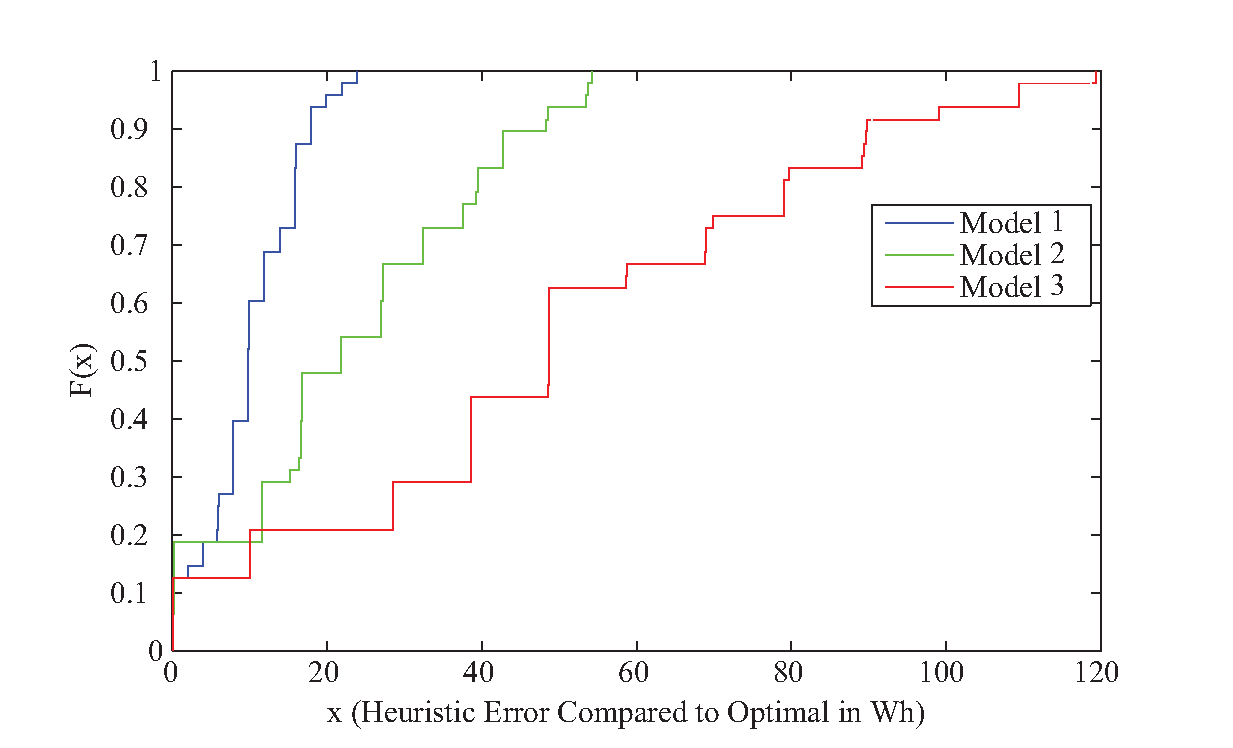
\includegraphics[width=0.5\textwidth]{pics/heuristicerror-touchedup.eps}
\caption{Empirical CDF of the difference between the cost offered by our heuristic compared to the optimal}
\label{fig:results5}
\end{figure}

We also ran experiments for each BTS model in which the electricity cost for the optimal as well as the heuristic solution (Algorithm 1) was computed. We assessed the performance of our heuristic by computing the difference (error) in the electricity cost of the two solutions. For statistical significance, we computed the error in our heuristic relative to the optimal solution over 48 different experiment runs for each BTS model. The resulting CDF of the heuristic error (in Wh) is plotted in Fig.~\ref{fig:results5}. We can see in Fig.~\ref{fig:results5} that our heuristic is quite close to the optimal solution most of the time, especially for the Model 1 and Model 2 BTS. For Model 3 BTS, while the error is comparatively larger, since the amount of savings with the optimal solution is quite high (Fig.~\ref{fig:case2:results2}), the heuristic will still result in significant energy savings.  

\subsection{Sensitivity of electricity cost savings to the resource pruning granularity} %We may have two states for a BTS: (i) 6+6+6, (ii) 3+3+3. Or, we may have three states: (i) 6+6+6, (ii) 4+4+4, and (iii) 2+2+2. How do the two-state and three-state resource pruning granularity settings comapre in terms of electricity cost savings? 
\label{subsec:case2:results:granularity} In our experimental results discussed so far, we have observed that going from a 6+6+6 configuration to a 2+2+2 configuration can save a significant amount of energy. Intuition suggests that going to a finer granularity of resource pruning should enable greater energy savings. We now present two cases that are different from the configuration considered so far. In the first case, we consider the ability to (de)activate TRXs in pairs, i.e., a site may be in one of three configurations at a given time: 6+6+6, 4+4+4 or 2+2+2. In the second case, we consider the ability to (de)activate each TRX on a site independently, i.e., at a given time, a site may be in one of six possible configurations. 

For the first case, a simple extension of the optimization model given in~\ref{subsec:case2:instantiate:multi-cell} as follows:

\begin{align}
\textit{minimize} \quad \sum_{j=1}^{m} x_j + y_j
\end{align}
subject to the following constraints:
\begin{align}
& \sum_{j=1}^m w_{i,j} = 1 \qquad \forall i \\
& w_{i,j} \leq c_{i,j} \qquad \forall i, j \\
& \sum_{i=1}^nw_{i,j}-\delta_1 +\epsilon \leq Mx_j \qquad \forall j \\
& \sum_{i=1}^nw_{i,j}-\delta_2 +\epsilon \leq My_j \qquad \forall j \\
& \sum_{i=1}^n w_{i,j} \le t_{max} \qquad \forall i \\
& w_{i,j}, x_j, y_j \in \{0,1\} \qquad \forall i, j%\\
\end{align}

Here, $x_j$ is a binary indicator variables that is 0 if the traffic at BTS $j$ is below $\delta1 - \epsilon$ and 1 otherwise. Similarly, $y_j$ is an indicator variable that is 0 if the traffic at BTS $j$ is below $\delta2$ and 1 otherwise.

For the second case, we present the following slightly different optimization formulation. Consider an integer variable $z_j$ which represents the number of TRXs active on BTS $j$. The power consumption at BTS $j$ may be given by $P_1 + p \sum_{i=1}^{n} w_{i,j} + \gamma z_j$, where p is the slope of the power consumption vs traffic volume curve. The RED-BL optimization problem for the multi-BTS setting in this case is:

\begin{align}
\textit{minimize} \quad \sum_{j=1}^{m} z_j
\end{align}
subject to the following constraints:
\begin{align}
& \sum_{j=1}^m w_{i,j} = 1 \qquad \forall i \\
& w_{i,j} \leq c_{i,j} \qquad \forall i, j \\
& \sum_{i=1}^nw_{i,j}-\delta_1 +\epsilon \leq Mz_j \qquad \forall j \\
& \sum_{i=1}^n w_{i,j} \le t_{max} \qquad \forall i \\
& w_{i,j} \in \{0,1\}; \quad z_j \in \{1,2,3,4,5,6\}\qquad \forall i, j%\\
\end{align}

The first constraint ensures that each call is handled at exactly one BTS. The second one ensures that a call is mapped to a BTS that may handle it. The third constraint ensures that $z_j$ picks a value at least equal to the minimum number of TRXs required at BTS $j$. Since the optimization is a minimization problem, the solver will pick $z_j$ to be exactly equal to the minimum number of TRXs required for the current traffic load. The fourth constraint is the capacity constraint on the BTS. The last set of constraints specify the domains of the decision variables.

In this scenario, we conducted simulation experiments where a re-optimization was performed every six minutes using model 1 BTS. The results of these experiments are given in Table~\ref{tab:granularityresults}. For all three BTS models, we see that going from a 2-state model to a 3-state model gives a relatively small increase in energy savings compared to the jump from 3-state to 6-state model.  

\begin{table}
\centering
\begin{tabular}{|c|c|c|c|}
\hline
Granularity & BTS Model 1 & BTS Model 2 & BTS Model 3\\
\hline 2-State & 5.38\% & 6.29\% &  14.94\% \\
\hline 3-State & 6.81\% & 7.73\% &  18.62\% \\
\hline 6-State & 14.69\% & 25.33\% &  33.69\% \\
\hline
\end{tabular}
\caption{Percentage electricity savings for different granularity of resource pruning}
\label{tab:granularityresults}
\end{table}


\subsection{Sensitivity of electricity cost savings to the margin of state-change damping} %Suppose that we are using a two-state resource pruning model. If $t_{max}$ is the call capacity of a 6+6+6 site, then the call capacity of the half-pruned site is $t_{max}/2$. If we deactivate TRXs immediately when the instantaneous call volume reaches $t_{max}/2$, we are likely to have many transitions due to short-term variations in call volume. We, therefore, wait until the instantaneous call volume is $t_{max}/2 - \epsilon$ before we switch to a $3+3+3$ configuration. The value of $\epsilon$ is a configurable parameter which can take a value from $0$ (very aggressive, lots of transients, perhaps more savings) to $t_{max}/2$ (very conservative, no transients, no savings either). How do the electricity cost savings vary with the value of $\epsilon$.
\label{subsec:case2:results:epsilon} If the value of $\epsilon$ in our optimization is set too aggressively, a BTS that is placed in low-power mode may have to be moved back to high-power mode soon afterwards due to short time scale variations in call volume. Theoretically, it is even possible that there may be several such back and forth transitions at a BTS. Such rapid state oscillations may be undesirable and to avoid these, the value of $\epsilon$ must be set at a safe value. Furthermore, if $\epsilon$ is set too aggressively, a BTS placed in low-power mode would be operating very close to it's \textit{new} and lower traffic capacity. If several calls arrive in a short time window, the BSC may not have sufficient time to bring the BTS back into high-power mode and, thus, some calls may be blocked. However, if $\epsilon$ is set too conservatively, the energy savings would be smaller. 

We carried out experiments to assess the impact of the value of $\epsilon$ on the energy savings achievable through RED-BL. For this purpose, we fixed the inter-optimization interval at 6 minutes and carried out RED-BL optimizations for all three BTS models. Furthermore, we considered a two-state BTS model, i.e., a BTS may be placed in either a 6+6+6 or a 2+2+2 configuration. The range of possible values for epsilon were 5, 10, 15 and 25. Since the traffic capacity of a 2+2+2 BTS is 44\footnote{The capacity of the 2+2+2 BTS is 3$\times$2$\times$8 = 48, but 4 channels were reserved by the operator for control and broadcast channels.}, any larger value for $\epsilon$ did not make sense. Figure~\ref{fig:case2:results6} shows the results. As expected, the percentage savings deplete almost linearly with increasing values of $\epsilon$.

\begin{figure}
\centering
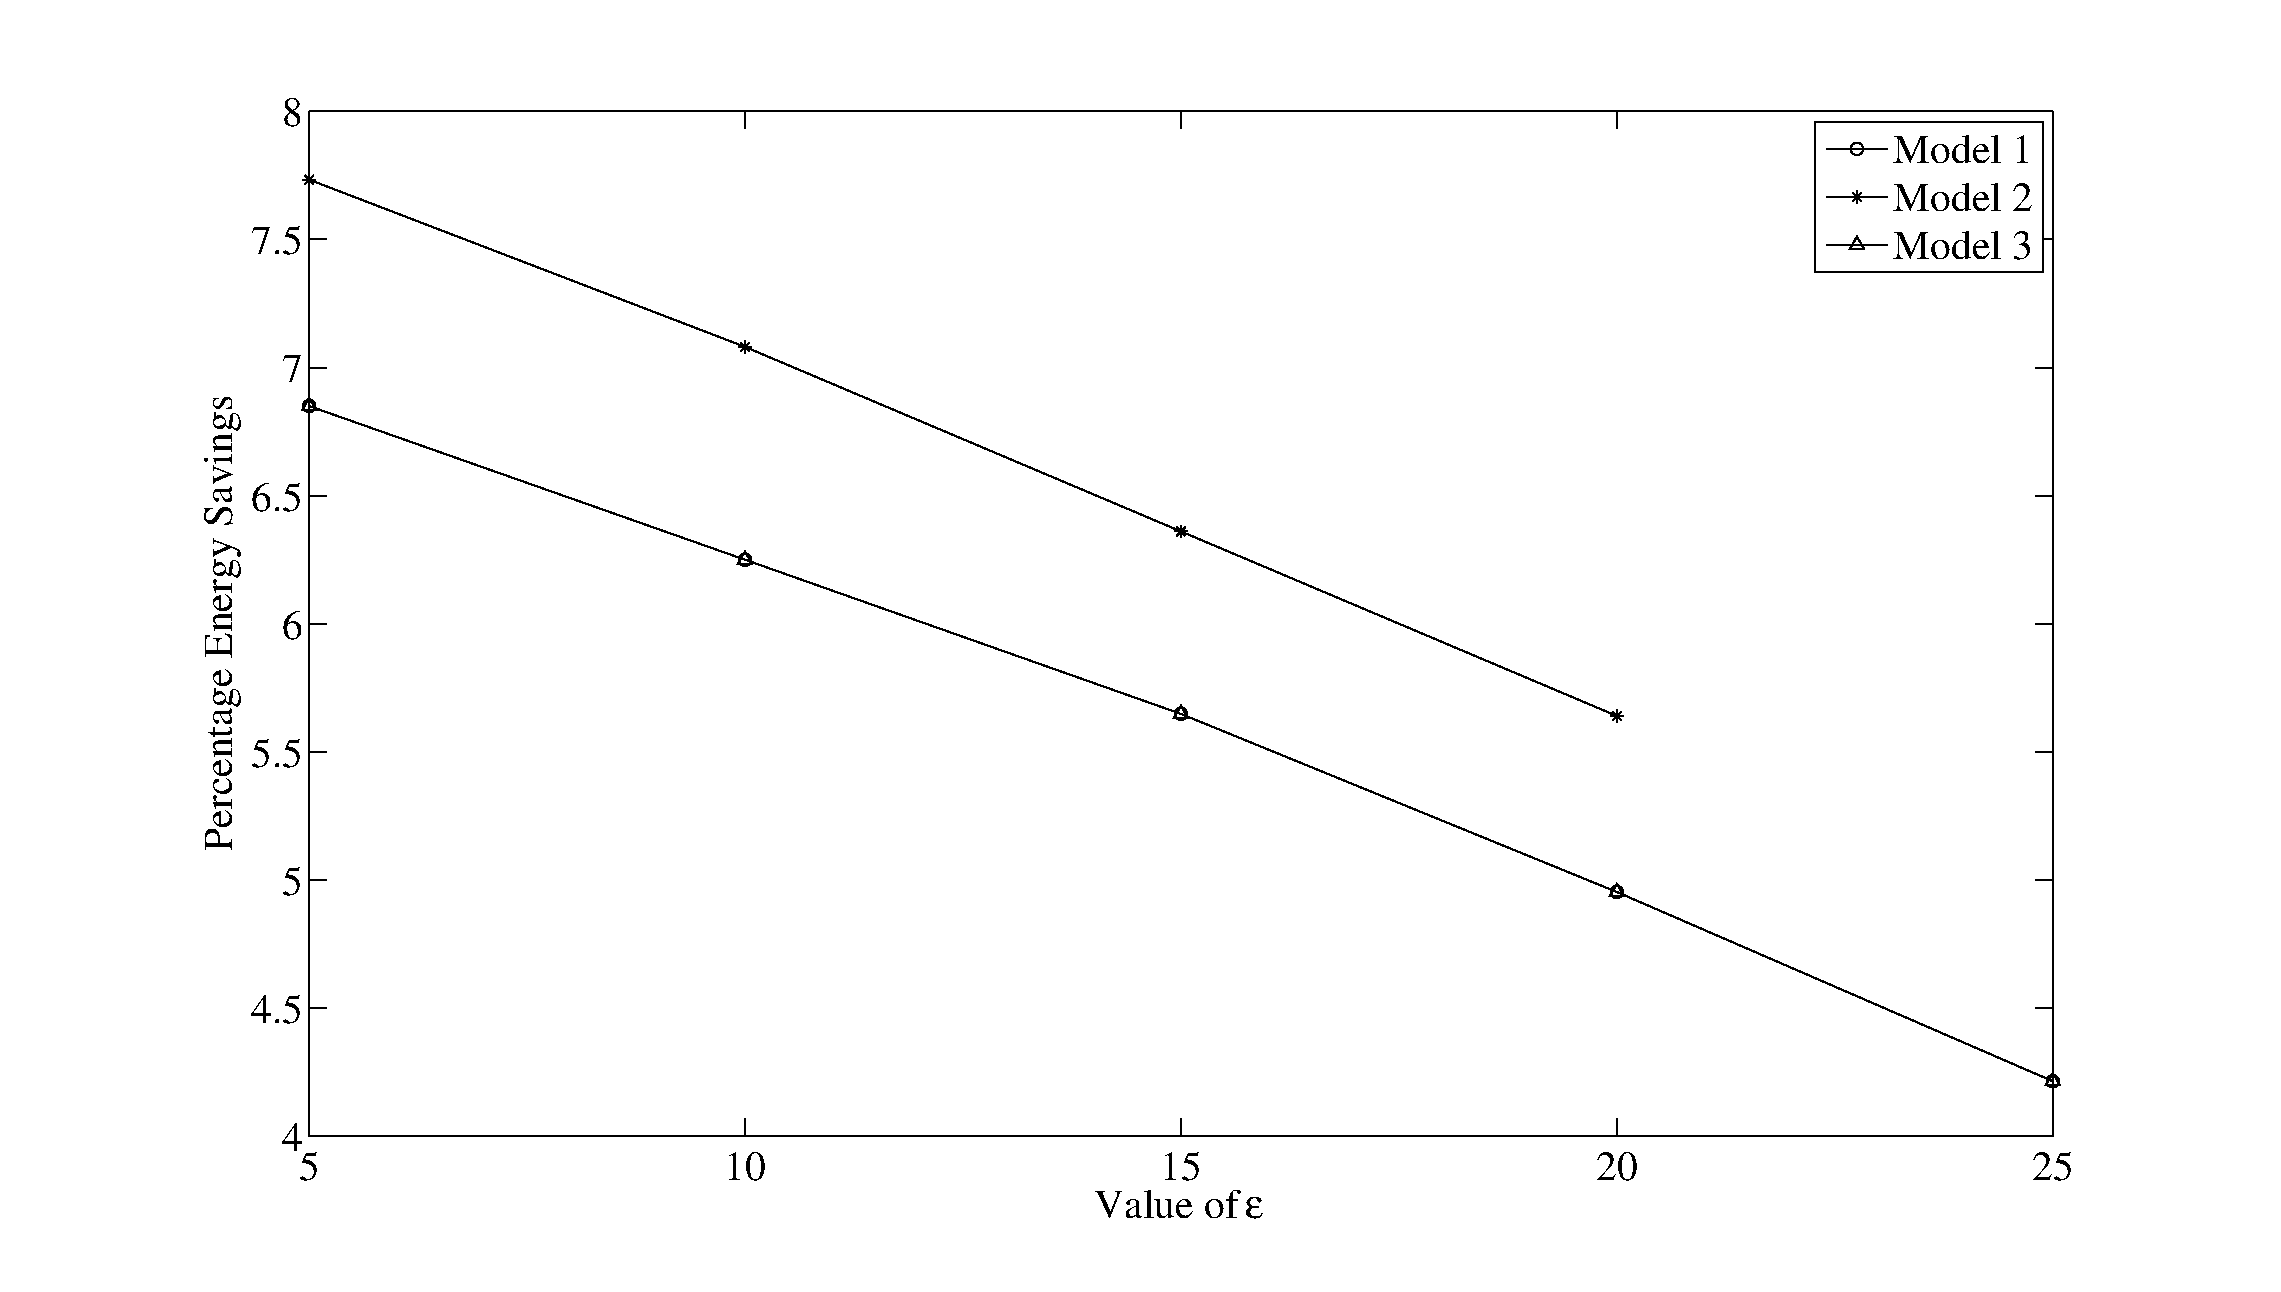
\includegraphics[width=0.8\textwidth]{pics/epsilonresults.eps}
\caption{The percentage energy savings for all three BTS models considered in this thesis vs the value of $\epsilon$, with a six minute inter-optimization interval}
\label{fig:case2:results6}
\end{figure}

\section{Discussion}
\label{sec:discuss:case2} In this chapter, we have seen an application of RED-BL to cellular networks. The nature of cellular networks is different compared to geo-diverse data centers (considered in the previous chapter) in the following ways:

\begin{itemize}
\item The workload (calls) has limited geographic flexibility and may only be handled at a few candidate resources (BTSs)
\item There is no geo-diversity in electricity prices
\end{itemize}

For resource pruning and workload relocation, we utilized two features built in to currently deployed equipment in the form of BTS power savings and network-controlled call handoff, respectively. Our simulation results show that jointly using workload relocation and resource pruning can bring in considerably higher gains in electricity savings compared to using resource pruning alone. Our results show the promising potential that RED-BL holds in greening current generation cellular networks.